\documentclass[aspectratio=169,mathserif]{beamer}

\usepackage[utf8]{inputenc}
\usepackage{graphicx}
\usepackage{tikz}
\usepackage{pgfplots}
\pgfplotsset{compat=newest}

\useoutertheme[numbering=fraction]{metropolis}
\useinnertheme{metropolis}
\usefonttheme{metropolis}
\usecolortheme{default}
\setbeamertemplate{title page}{
\begin{minipage}[b][\paperheight]{\textwidth}
\ifx\inserttitlegraphic\@empty\else\usebeamertemplate*{title graphic}\fi
\vfill%
\ifx\inserttitle\@empty\else\usebeamertemplate*{title}\fi
\ifx\insertsubtitle\@empty\else\usebeamertemplate*{subtitle}\fi
\usebeamertemplate*{title separator}
\ifx\beamer@shortauthor\@empty\else\usebeamertemplate*{author}\fi
\ifx\insertinstitute\@empty\else\usebeamertemplate*{institute}\fi
\ifx\insertdate\@empty\else\usebeamertemplate*{date}\fi
\vfill
\vspace*{1mm}
\end{minipage}
}

%%% Local Variables:
%%% mode: latex
%%% TeX-master: t
%%% End:

\usepackage{appendixnumberbeamer}
\usepackage{FiraSans}

\usepackage[longnamesfirst]{natbib}
\usepackage{amsmath, amsthm, mathtools}
\usepackage{booktabs}

\title{Wealth Taxation through the Lens of the Aiyagari Model}
\author{Fabian Greimel}
\date{June 2025}

\begin{document}

\frame{\titlepage}

\section{\citet{guvenen2023use}}

\begin{frame}{Capital income taxes vs wealth taxes}
    \begin{itemize}
        \item comparing after-tax wealth
        \begin{align*}
            a_{i}^{\text{after-tax}} &= a_{i} + (1 - \tau_{k}) \cdot r \cdot a_{i} = (1+r)\cdot a_i - \tau_{k} r \cdot a_{i}\\
            a_{i}^{\text{after-tax}} &= (1 - \tau_{a}) \cdot a_{i} + r \cdot a_{i} = (1+r) \cdot a_i - \tau_{a} \cdot a_{i}\\
        \end{align*}
        \item what if $\tau_a = r \tau_k$?
    \end{itemize}
\end{frame}

\begin{frame}{Table 1: Kourtney K. $(r_{Ko} = 0\%)$ vs Kim K. $(r_{Ki} = 20\%)$}
    \begin{table}
        \centering
        \begin{tabular}{lcccrr}
            \toprule
            & \multicolumn{2}{c}{Capital income tax} & \multicolumn{2}{c}{Wealth tax} \\
            \cmidrule(lr){2-3} \cmidrule(lr){4-5}
            & Kourtney & Kim & Kourtney & Kim \\
            \midrule
            Rate of return & $0\%$ & $20\%$ & $0\%$ & $20\%$ \\
            Wealth & 100 M & 100 M & 100 M & 100 M \\
            Pretax income & 0 & 20 M & 0 & 20 M \\
            Tax liability & 0 & 5 M & 2.5 M & 2.5 M \\
            After-tax rate of return & 0\% & 15\% & $-2.5\%$ & 17.5\% \\
            After-tax wealth & 100 M & 115 M & 97.5 M & 117.5 M \\
            \bottomrule
        \end{tabular}
    \end{table}

   \centering \structure{What will happen in the long-run?}
\end{frame}

\begin{frame}{Recall: Aiyagari}
    \begin{align*}
    V(a, y) &= \max_{c, a'} \left\{ u(c) + \beta \mathbb{E}[V(a', y')] \right\} \\
    &\begin{aligned} \text{s.t. } & c + a' = (1 + r) a + y
        \\
       % &\textcolor{red}{r = r(a) + \sigma(a) \cdot x} \\
        &y \sim \text{some Markov Chain} \\
        &a' \geq \underline{a}
    \end{aligned}
    \end{align*}
    where
    \begin{itemize}
        \item $a$ is current assets,
        \item $y$ is risky labor income,
        \item $r$ is the interest rate,
        \item $\beta$ is the discount factor.
    \end{itemize}
\end{frame}

\begin{frame}{Skills}
    \begin{itemize}
        \item entrepreneurial skill
        \begin{equation*}
            \log(z_{\text{child},i})
            = \rho_z\,\log(z_{\text{parent},i}) 
               + \varepsilon_{z,i}
        \end{equation*}
        \item labor productivity
        \begin{align*}        
            \log w_{i j}
                &= \underbrace{\kappa_i}_{\text{permanent}}
                   + \underbrace{g(j)}_{\text{life cycle}}
                   + \underbrace{e_{i j}}_{\text{AR(1)}}                \\
%            e_{i j}
%                &= \rho_e\,e_{i,j-1} + \nu_{i j}                           \\
            \kappa_{\text{child},i}
                &= \rho_{\kappa}\,\kappa_{\text{parent},i} 
                   + \varepsilon_{\kappa,i}                                
        \end{align*}    
    \end{itemize}
\end{frame}

\begin{frame}{Aiyagari with lifecycle, entrepreneurs and labor choice}
    \begin{align*}
    V_j(a, e) &= \max_{c, \ell, a', b} \left\{\phi_j u(c, (1-\ell)) + (1-\phi_j)v(b) + \beta \mathbb{E}[V(a', e')] \right\} \\
    &\begin{aligned} \text{s.t. } 
        & \log w = \kappa + g(j) + e \\
        & c + a' = \textcolor{red}{\pi(a, z)} + \ell \cdot w \\
        & e \sim \text{some Markov Chain} \\
        &a' \geq \underline{a}(z) \\
        &\kappa, z \text{ given}
    \end{aligned}
    \end{align*}
    where
    \begin{itemize}
        \item $\ell$, $\phi_j$, $v(b)$
        \item $z, \kappa$
        \item $\pi(a, z)$
    \end{itemize}
\end{frame}

\begin{frame}{Production side}
    \begin{itemize}
        \item Final output: $Y = F(K_e, X)$, where $K_e$ is entrepreneurial capital and $X$ is the intermediate good.
        \item Intermediate good $X$ is produced by specialized firms using labour and technology.
        \item Bonds market: agents trade risk-free bonds $B$ at interest rate $r_b$ to finance investment and smooth consumption.
    \end{itemize}
\end{frame}


%\begin{frame}{Tax reform}
%    \begin{itemize}
%        \item Reform design: replace the capital‐income tax $\tau_k$ with a wealth tax $\tau_a$
%        \item Revenue‐neutral calibration: set 
%              $\displaystyle \tau_a = \bar r\,\tau_k$, 
%              where $\bar r$ is the average return
%        \item Under the wealth tax, effective rates vary inversely with individual $r_i$
%        \item Distributional impact: high‐return agents pay less under $\tau_k$ but more under $\tau_a$
%    \end{itemize}
%\end{frame}

\subsection{Tax reform}

\begin{frame}{Table 5}
    \centering
    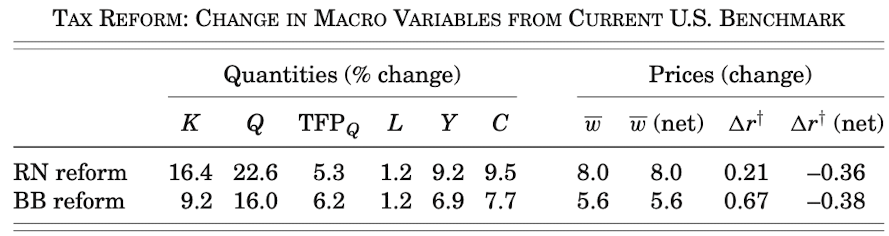
\includegraphics[scale = 0.4]{GKKOC_Tab5.png}
\end{frame}

\begin{frame}{Measuring welfare effects}

    \begin{itemize}
        \item compare two steady states
        \begin{itemize}
            \item optimal policy functions $\tilde c(a, y)$, $\hat c(a, y)$
            \item optimal expected value
            $$\tilde V_0 = \mathbb{E}_0 \sum_{j=0}^{J-1} \beta^j u(\tilde c_j), \qquad \hat V_0 = \mathbb{E}_0 \sum_{j=0}^{J-1} \beta^j u(\hat c_j)$$
        \end{itemize}
        \item how what relative income change $\textcolor{red}{\Delta}$ (uniform across all states and ages $j$) would equalize these two values?
        \begin{equation*}
            \mathbb{E}_0 \sum_{j=0}^{J-1} \beta^j u(\tilde c_j) \stackrel{!}{=} \mathbb{E}_0 \sum_{j=0}^{J-1} \beta^j u(\textcolor{red}{\Delta} \hat c_j)
        \end{equation*}
    \end{itemize}
\end{frame}


\begin{frame}{Table 6}
    \centering
    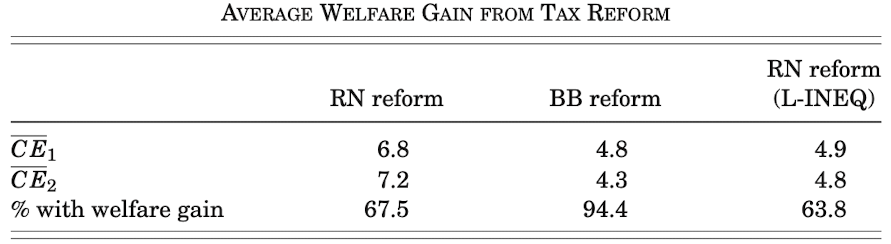
\includegraphics[scale = 0.4]{GKKOC_Tab6.png}
\end{frame}


\begin{frame}{Table 7}
    \centering
    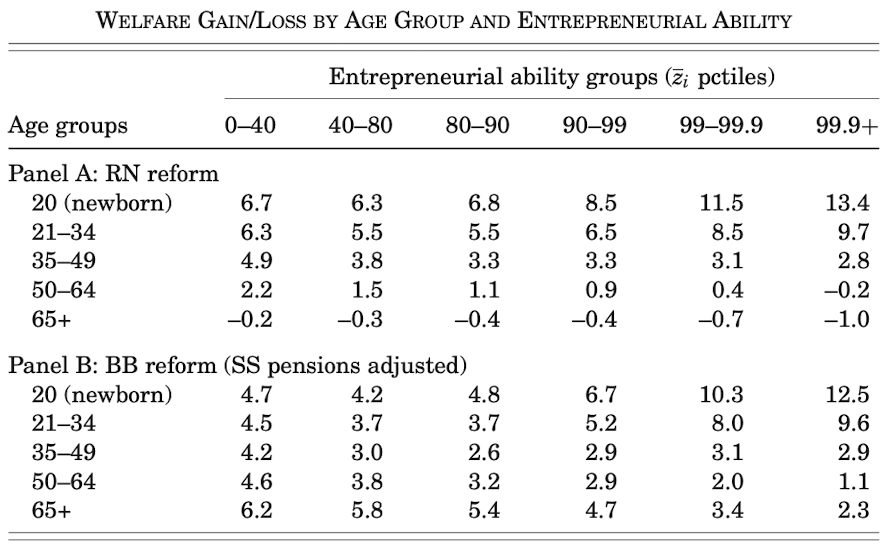
\includegraphics[scale = 0.4]{GKKOC_Tab7.png}
\end{frame}

\begin{frame}{Tax reform: Summary}
    \begin{itemize}
        \item Wealth tax is less distortive than capital income tax (use-it-or-lose-it)
        \item Welfare gains relatively evenly distributed%, with all newborn cohorts preferring the wealth tax regime.
        %\item Indexing pensions to average wages (BB reform) reduces average welfare gains but spreads benefits to the vast majority of the population.
        %\item The welfare gains from the wealth tax remain positive and robust even under lower top-end wealth inequality calibrations.
    \end{itemize}
\end{frame}

\section{\cite{boar2023income-or-wealth}}

\begin{frame}{Overview}
    \begin{itemize}
        \item Capital income tax is better than wealth tax
        \item Losses from misallocation are much smaller
        \item 
        \item \cite{guvenen2023use}: capital usage is tied to entrepreneurial skill
        \item \cite{boar2023income-or-wealth}: unskilled people can rent capital to firm
        \item Transition dynamics vs Steady states
        \item \cite{boar2023income-or-wealth} use simpler model
    \end{itemize}
    
\end{frame}
\begin{frame}{Model}

    \begin{itemize}
        \item Infinite horizon, no deaths/births
        \item capital can be used twice by entrepreneurs; income is given by
        \begin{equation*}
            i_t =  w_t e_t (1 - \ell_t) + r_{t-1} a_t + \pi_t(a_t, z_t)
        \end{equation*}
        \item ($\implies$ all entrepreneurs produce?)
        \item firm \& entrepreneurs produce the same good
        \item entrepreneurs provide only 37\% of output
       
    \end{itemize}
\end{frame}

\begin{frame}{Table 2}
    \centering
    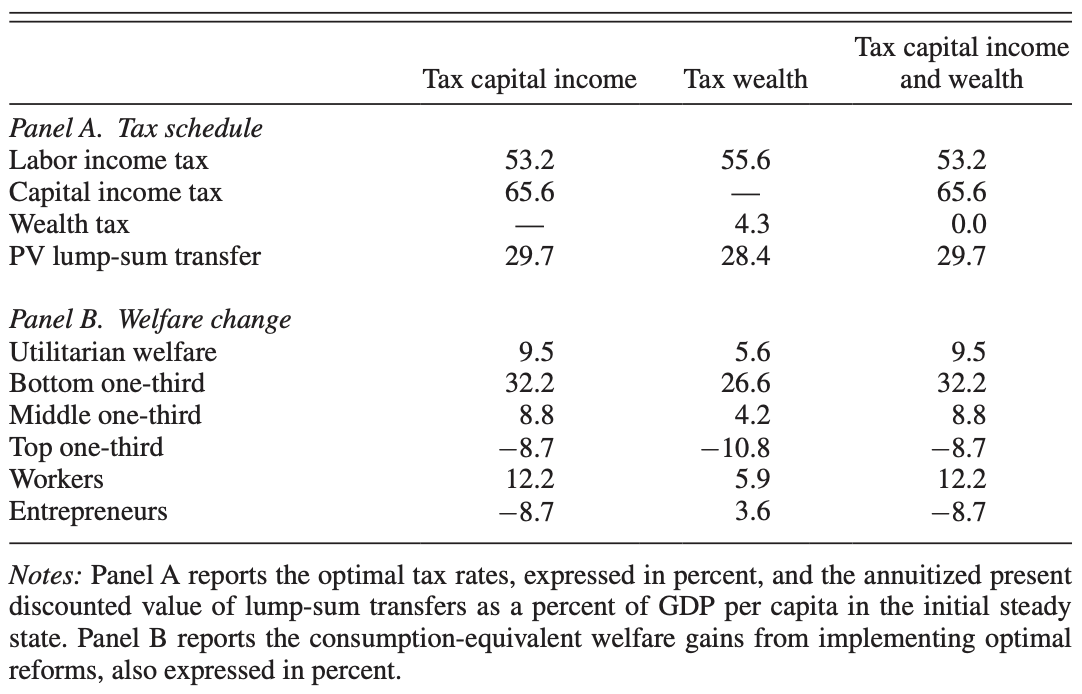
\includegraphics[scale = 0.6]{BM_Tab_2.png}
\end{frame}

\begin{frame}{Table 3}
    \centering
    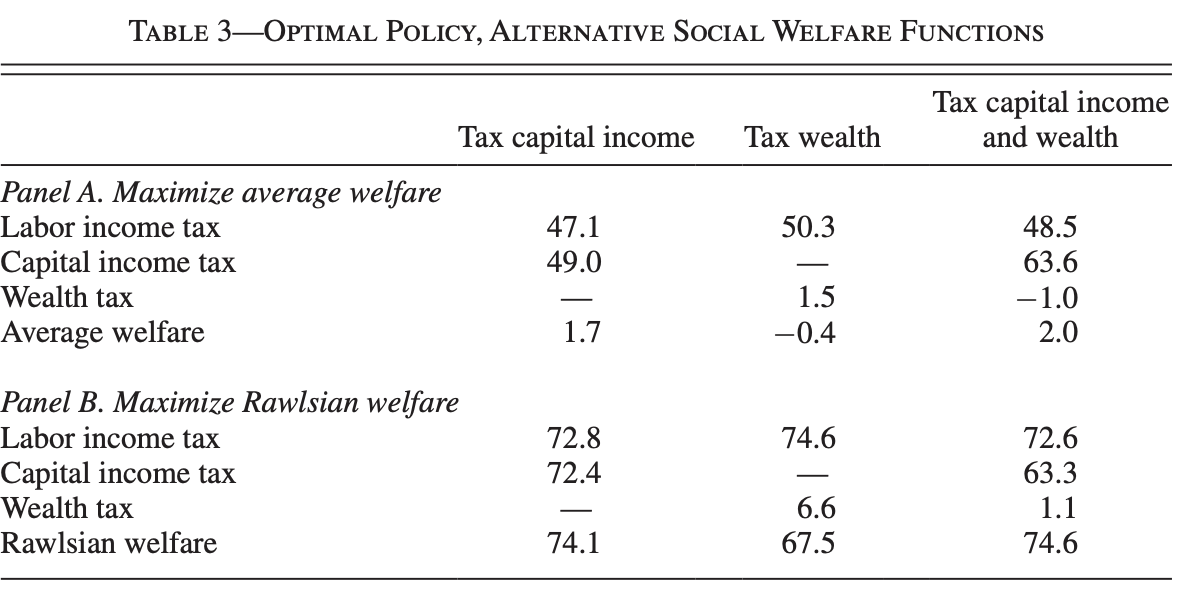
\includegraphics[scale = 0.6]{BM_Tab_3.png}
\end{frame}

\begin{frame}{Figure 1}
    \centering
    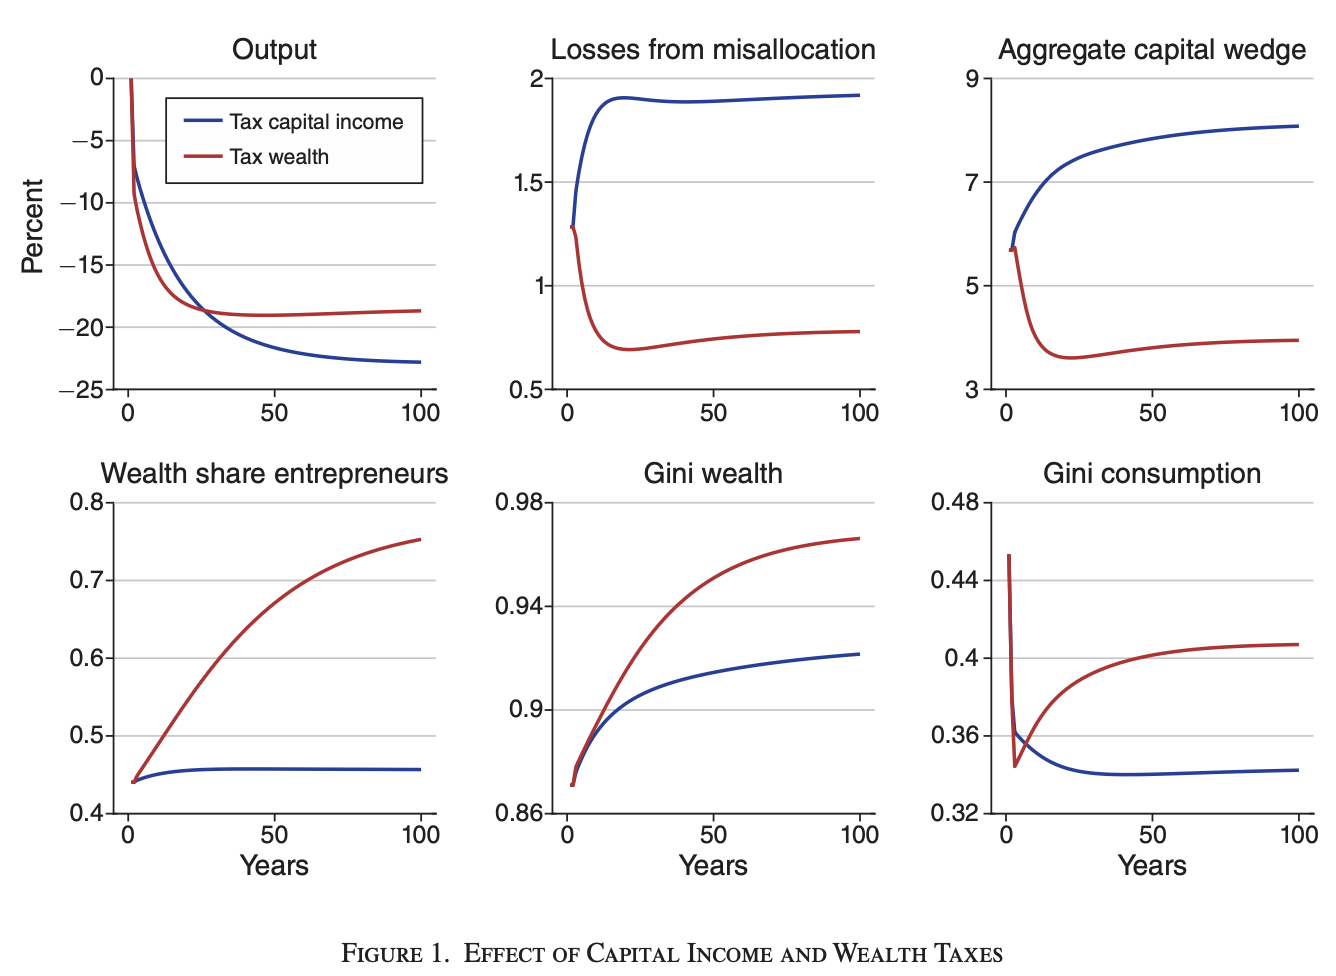
\includegraphics[scale = 0.45]{BM_Fig_1.png}
\end{frame}


\begin{frame}{Criticisms}
    \begin{itemize}
        \item measuring welfare changes along the transition is good, but
        \begin{itemize}
            \item why don't show steady-state comparison first? (does the transition flip the result?)
            \item why don't let people die (perpetual youth)
        \end{itemize}
        \item simple income process: permanent/persistent vs transitory shocks is standard
        \item lacking explantion of differences vs \cite{guvenen2023use}
        \item capital can be used twice by entrepreneurs
        \item entrepreneur's production is perfectly substitutable
        \item don't decompose welfare changes
    \end{itemize}
    
\end{frame}

\begin{frame}{Insights}
    \begin{itemize}
        \item measure of welfare change matters
        \begin{equation*}
            \int \frac{\Delta_i^{1 - x}}{1-x} di
        \end{equation*}
        \begin{itemize}
            \item \citet{guvenen2023use} use $x=0$
            \item \citet{boar2023income-or-wealth} use $x = \sigma$ (CRRA parameter) 
        \end{itemize}
        \item $x$ captures preference for (in)equality
     
    \end{itemize}
    
\end{frame}
\bibliographystyle{ecta}
\bibliography{../inequality}

\end{document}